\documentclass{beamer}
%[aspectratio=169]   \usepackage[czech]{babel}
\usepackage{apo-lecture-cz}
\usepackage{pdfpages}
\usepackage{pdfcomment}
\usepackage{listings}
\usepackage{array,multirow}

\subtitle{Lekce 05. Zřetězené zpracování\\Pipelining}
\author{Pavel Píša \phantom{xxxxxxx} Petr Štěpán \\ \small\texttt{pisa@fel.cvut.cz}\phantom{xxxx}\small\texttt{stepan@fel.cvut.cz}}
\begin{document}

\maketitle

\section{Zřetězené zpracování}

\begin{frame}
\frametitle{Cíl dnešní přednášky}

\begin{itemize}
 \item Navrhnout úpravy procesoru z lekce 3 tak, aby využíval zřetězené zpracování (pipelining) a tím ho bylo možné zrychlit
 \item Stále uvažujeme následující instrukce: \texttt{add}, \texttt{sub}, \texttt{and}, \texttt{or}, \texttt{slt}, \texttt{addi}, \texttt{lw}, \texttt{sw}, a \texttt{beq}
 \item Kódování instrukcí také zůstává
\end{itemize}

\begin{table}
\footnotesize
\begin{tabular}{|m{0.4cm}|m{0.4cm}|m{1.0cm}|m{1.0cm}|m{0.4cm}|m{1.0cm}|m{1.0cm}|m{1.0cm}|m{0.4cm}|m{1.0cm}|}\hline
Typ & 31 & 30...25 & 24...21 & 20 & 19...15 & 14...12 & 11...8 & 7 & 6...0 \\ \hline
R & \multicolumn{2}{c|}{ fnct7 } & \multicolumn{2}{c|}{ rs2 } & rs1 & fnct3 &\multicolumn{2}{c|}{ rd } & opcode\\ \hline
I & \multicolumn{4}{c|}{ imm[11:0] } & rs1 & fnct3 &\multicolumn{2}{c|}{ rd } & opcode\\ \hline
S & \multicolumn{2}{c|}{ imm[11:5] } & \multicolumn{2}{c|}{ rs2 } & rs1 & fnct3 &\multicolumn{2}{c|}{ imm[4:0] } & opcode\\ \hline
B & imm [12] & imm [10:5]  & \multicolumn{2}{c|}{ rs2 } & rs1 & fnct3 & imm[4:1]& imm [11] & opcode\\ \hline
U & \multicolumn{6}{c|}{ imm[31:12] }  & \multicolumn{2}{c|}{ rd } & opcode\\ \hline
J & imm [20] & \multicolumn{2}{c|}{ imm[10:1] } & imm [11] & \multicolumn{2}{c|}{ imm[19:12] } & \multicolumn{2}{c|}{ rd } & opcode\\ \hline
\end{tabular}
\end{table}

\end{frame}

\begin{frame}
\frametitle{Jednocyklový procesor s pamětí (z přednášky 3)}

\includegraphics[width=0.95\textwidth]{single_cpu.pdf}
\end{frame}

\begin{frame}
\frametitle{Propustnost jednocyklového procesoru je omezená}

\begin{itemize}
 \item Maximum instrukcí za sekundu $IPS = IC / T = IPC_{avk} \cdot f_{clk}$
 \item Omezené nejdelší dobou průchodu signálu od zapamatované hodnoty na vstup zápisu do paměti, registru  (critical path)
 \item V našem návrhu omezení z kritické cesty instrukce \texttt{lw}
\end{itemize}


\includegraphics[width=0.92\textwidth]{cpu-time.pdf}
\end{frame}

\begin{frame}
\frametitle{Kritická cesta omezující propustnost}

$f_{clk} = 1 / T_{C}$ kde $T_{C}$ je perioda hodin/čas na zpracování jednoho cycklu

\vskip 2 mm

$T_{C} = t_{PC} + t_{Mem} + t_{RFread} + t_{ALU} + t_{Mem} + t_{Mux} + t_{RFsetup}$

\vskip 2 mm

Uvažujeme následující zpoždění a časové požadavky

\vskip 2 mm

\begin{tabular}{l c r}
$t_{PC}$ & = & $30$ ns \\
$t_{Mem}$ & = & $300$ ns \\
$t_{RFread}$ & = & $150$ ns \\
$t_{ALU}$ & = & $200$ ns \\
$t_{Mux}$ & = & $20$ ns \\
$t_{RFsetup}$ & = & $20$ ns \\
\end{tabular}

\vskip 2 mm

tak $T_{C} = 1020$\,ns $\rightarrow$ $f_{clk max} = 980$\,kHz

\vskip 2 mm

$IPS = IC / T = IPC_{avg} \cdot f_{clk}$

\vskip 2 mm

$IPS = 1 \cdots 980e3 = 980\,000$ instrukcí za sekundu

\end{frame}

\begin{frame}
\frametitle{Rozdělení načítání a vykonávání instrukcí}

\begin{itemize}
 \item Načtení instrukce a čtení z paměti ($2 \times t_{Mem}$) představuje obvykle značnou část celkové doby potřebné na cyklus
 \item Ke zkrácení doby cyklu přispěje, pokud je instrukce načtena již v předchozím cyklu
\end{itemize}

\vskip 2 mm

{
\centering

\includegraphics[width=0.8\textwidth]{cpu_ifetch_exe.pdf}
}

\vskip 2 mm

\begin{enumerate}
 \item Načtení instrucke (instrukcion fetch) a zvýšení čítače instrukcí $PC = PC + 4$
 \item Vlastní vykonání (execution) instrukce až v následujícím cyklu
\end{enumerate}

\end{frame}

\begin{frame}
\frametitle{Úprava procesoru pro přednačítání instrukcí}

\includegraphics[width=0.95\textwidth]{cpu_clock.pdf}
\begin{itemize}
 \item $\downarrow$ v obrázku představuje hodinový vstup aktivní na vzestupnou hranu hodinového signálu
\end{itemize}

\end{frame}

\begin{frame}
\frametitle{Kritická cesta v případě přednačítání}

Pro již dříve uvažované parametry

\vskip 2 mm

\begin{tabular}{l c r m{1 cm} l c r}
$t_{PC}$ & = & $30$ ns & & $t_{Mem}$ & = & $300$ ns \\
$t_{RFread}$ & = & $150$ ns  & & $t_{ALU}$ & = & $200$ ns \\
$t_{Mux}$ & = & $20$ ns  & & $t_{RFsetup}$ & = & $20$ ns \\
\end{tabular}

\vskip 2 mm

\begin{itemize}
 \item Uvažujeme $T_{C_{fetch}} =  t_{PC} + t_{Mem}$ probíhající paralelně s výkonáváním instrukce
 \item $T_{C_{exec}} = t_{RFread} + t_{ALU} + t_{Mem} + t_{Mux} + t_{RFsetup}$
\end{itemize}

po dosazení

\begin{itemize}
 \item Uvažujeme $T_{C_{fetch}} =  30 + 300 = 330$\,ns
 \item $T_{C_{exec}} = 150 + 200 + 300 + 20 + 20 = 690$\,ns
 \item $T_{C_{fetch}} < T_{C_{exec}}$ tedy $T_{C} = T_{C_{exec}} = 690$\,ns
 \item $\rightarrow f_{C} = 1.45$\,MHz $\rightarrow IPS = 1\,450\,000$
\end{itemize}

Bez úprav dojde ke zpoždění skolových instrukcí (\texttt{beq}), viz poději

\end{frame}

\section{Pětistupňová pipeline}

\begin{frame}
\frametitle{Zřetězené vykonávání instrukcí -- pipelining}

Budeme uvažovat rozdělení vykonávání instrukcí do pěti stupní (stages).

\vskip 2 mm

{
\centering

\includegraphics[width=0.9\textwidth]{cpu_pipe_stages.pdf}
}

\begin{enumerate}
 \item \textbf{IF} načtení instrukce \textbf{Instruction Fetch} -- přivedení \textbf{PC} na adresový vstup paměti, načtení instrukce a paralelně příprava $PC = PC + 4$
 \item \textbf{ID} dekódování instrukce \textbf{Instrukction Decode} -- dekódování operačního znaku (opcode), přímého operand a načtení registrů podle polí \texttt{rs1} a \texttt{rs2}
 \item \textbf{EX} vykonání instrukce \textbf{EXecution} -- provedení požadované funkce, průchod hodnot registrů a konstant ALU
 \item \textbf{MEM} paměťové přístupy \textbf{MEMory} -- pokud je požadovaný, proběhne v tomto stupni zápis (\textbf{sw}) nebo čtení (\textbf{lw}) paměti
 \item \textbf{WB} aktualizace registrů \textbf{WriteBack} -- zápis výsledku do pole registrů pro meziregistrové instrukce a paměti
\end{enumerate}

\end{frame}

\begin{frame}
\frametitle{Překrývající se zřetězené vykonávání instrukcí}

\includegraphics[width=0.9\textwidth]{cpu_pipe_inst_flow-cz.pdf}

$\tau = max{\left\lbrace \tau_i \right\rbrace}^k_{i=1}$,  kde $\tau_i$ je zpožení v jednotlivých stupních

Vykonání $n$ instrukcí pro $k$ stupňové zřetězené zpracování trvá
$$T_{k,n} = k \cdot \tau + (n - 1) \tau$$
Zrychlení (Speedup)
\hskip 7mm
$S_{k,n} = \frac{T_{1,n}}{T_{k,n}} = \frac{n k \tau}{k \tau + (n - 1) \tau}$
\hskip 7mm
$\lim_{n \rightarrow \infty} S_k = k$

\end{frame}

\begin{frame}
\frametitle{Jednocyklový procesor (z přednášky 3) -- datová cesta}

\includegraphics[width=0.95\textwidth]{cpu_nopipe.pdf}
\end{frame}

\begin{frame}
\frametitle{Zřetězený pětistupňový návrh -- datová cesta}

\includegraphics[width=0.95\textwidth]{cpu_pipe.pdf}
\end{frame}

\begin{frame}
\frametitle{Zřetězený pětistupňový návrh včetně řídicí jednotky}

\includegraphics[width=0.95\textwidth]{cpu_ctrl_pipe.pdf}
\end{frame}

\section{Vznik a ošetření hazardů}

\begin{frame}
\frametitle{Datové a řídící hazardy a jejich řešení}
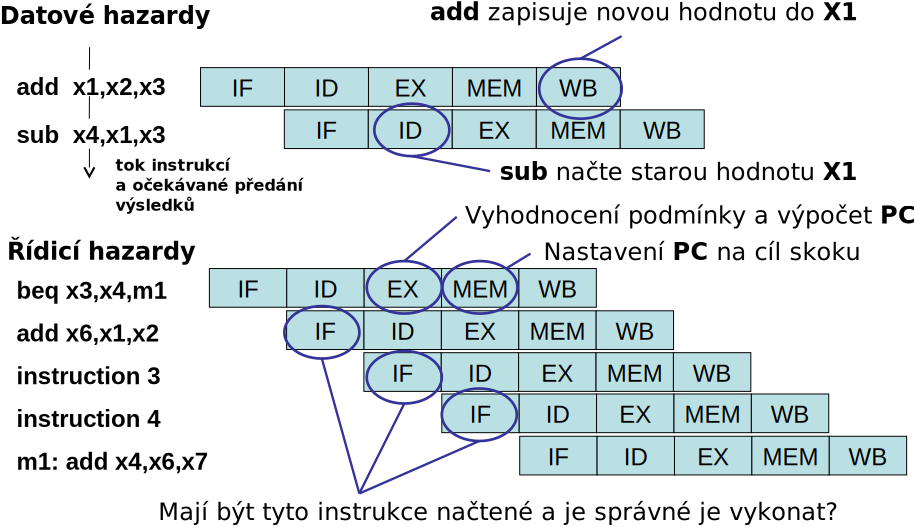
\includegraphics[width=0.95\textwidth]{hazard_kinds-cz.pdf}
\end{frame}

\begin{frame}
\frametitle{Zdroj datových hazardů}
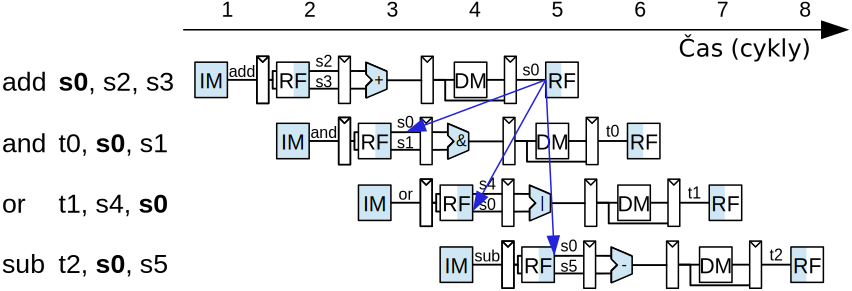
\includegraphics[width=0.95\textwidth]{hazard_data-cz.pdf}

\vskip 2 mm

\begin{itemize}
 \item K zápisníkové paměti (register file) se přistupuje ze dvou stupňů (Decode, WriteBack) --
       zápis se uskutečňuje v první půli cyklu, čtení v druhé $\Rightarrow$ v instrukci sub pro vstop \textbf{s0} hazard nevzniká
 \item Čtení-po-zápisu (Read After Write -- RAW) hazard vzniká u instrukcí
       \textbf{and} a \textbf{or} při čtení \textbf{s0} v cyklech 3 a 4
 \item Jak zamezit takovému hazardu bez degradace propustnosti pipeline?
\end{itemize}

\end{frame}


\begin{frame}
\frametitle{Datový hazard v instrukci "and" sledovaný v simulátoru}
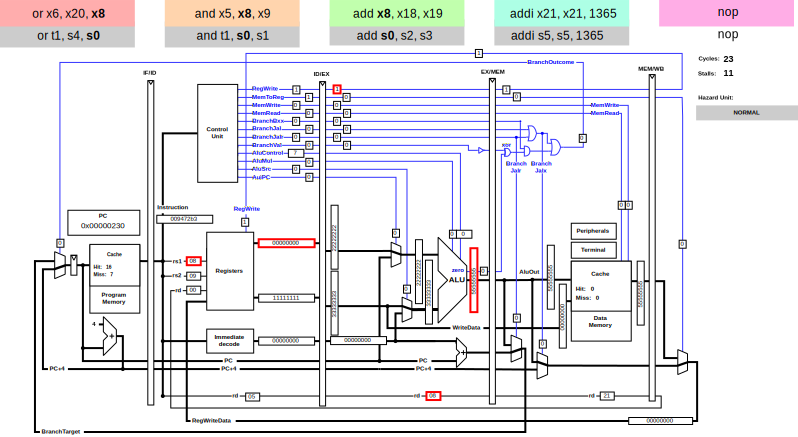
\includegraphics[width=0.95\textwidth]{hazard_qtrvsim.pdf}

{\tiny
QtRvSim \url{https://github.com/cvut/qtrvsim}
}

{\Tiny
\url{https://gitlab.fel.cvut.cz/b35apo/stud-support/-/blob/master/seminaries/qtrvsim/hazards-from-lecture/alu-hazards.S}
}

\end{frame}

\begin{frame}
\frametitle{Vyřešení datového hazardu pozastavením (stall)}
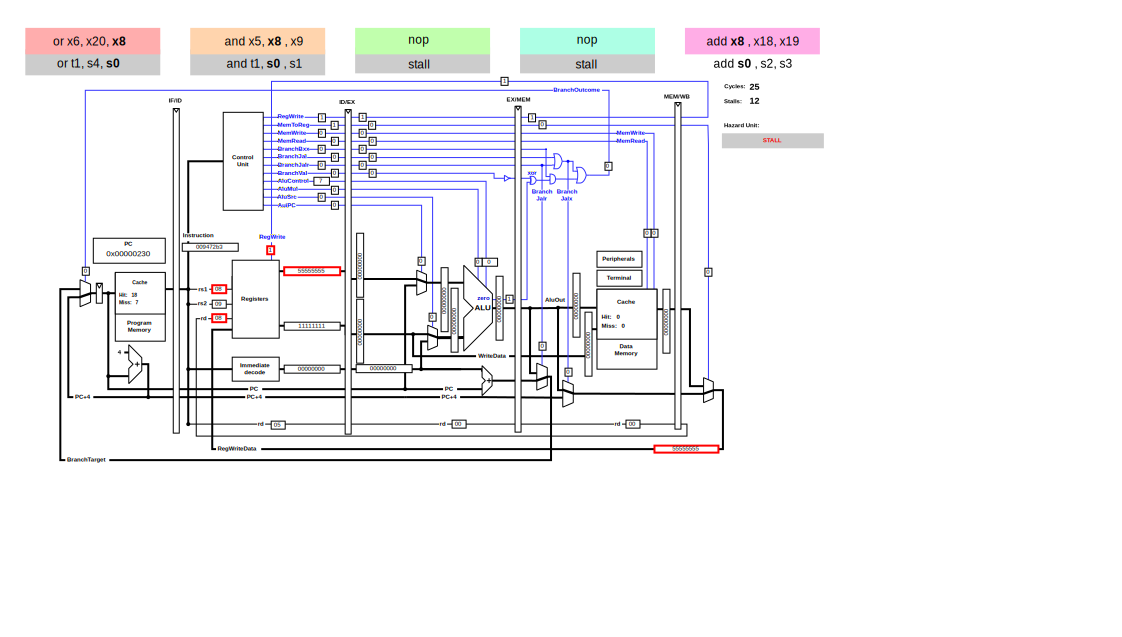
\includegraphics[width=0.95\textwidth]{hazard_stall_qtrvsim.pdf}

{\tiny
QtRvSim \url{https://github.com/cvut/qtrvsim}
}

{\Tiny
\url{https://gitlab.fel.cvut.cz/b35apo/stud-support/-/blob/master/seminaries/qtrvsim/hazards-from-lecture/alu-hazards.S}
}

\end{frame}


\begin{frame}
\frametitle{Rešení datových hazardů přeposíláním (forwarding)}
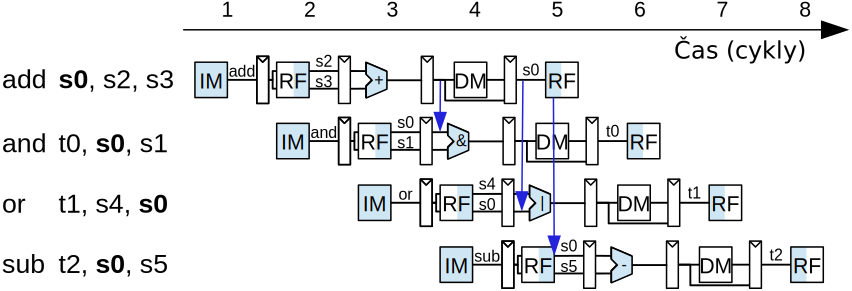
\includegraphics[width=0.85\textwidth]{forward_data-cz.pdf}

\begin{itemize}
 \item pokud je výsledek k dispozici (vypočítaný) před vykonáním následující instrukce/í,
       která/é vyžadují výsledek, tak je možné datový hazard vyřešit přeposláním hodnoty
 \item K datovému hazardu v uvažovaném návrhu dochází, pokud některý zdrojový registr
       (\textbf{rs1}, \textbf{rs2}) v stupni \textbf{EX} odovídá cílovému registru
       ve stupni \textbf{MEM} nebo \textbf{WB} (vyjma X0/zero)
 \item Čísla registrů z daných stupňů jsou přivedena na jednotku řešení hazardů (Hazard Unit -- HU)
\end{itemize}

\end{frame}

\begin{frame}
\frametitle{Zopakovaný předchozí návrh a příprava na přeposílání}

\includegraphics[width=0.95\textwidth]{noforward_data.pdf}

Je potřeba znát předchozí \textbf{A1} (\textbf{rs1}) a \textbf{A2} (\textbf{rs2}) v \textbf{EX}.
Signály \textbf{RegWrite} z \textbf{MEM} a \textbf{WB} musí být také monitorované aby potvrzovaly,
že registr určený \textbf{WriteReg} v \textbf{MEM} a \textbf{WB} je opravdu zapisovaný.

\end{frame}

\begin{frame}
\frametitle{Návrh procesoru s přeposíláním z MEM a WB do EX}

\includegraphics[width=0.95\textwidth]{forward_hazard.pdf}
\end{frame}

\begin{frame}
\frametitle{QtRvSim -- datové hazardy řešené přeposíláním}
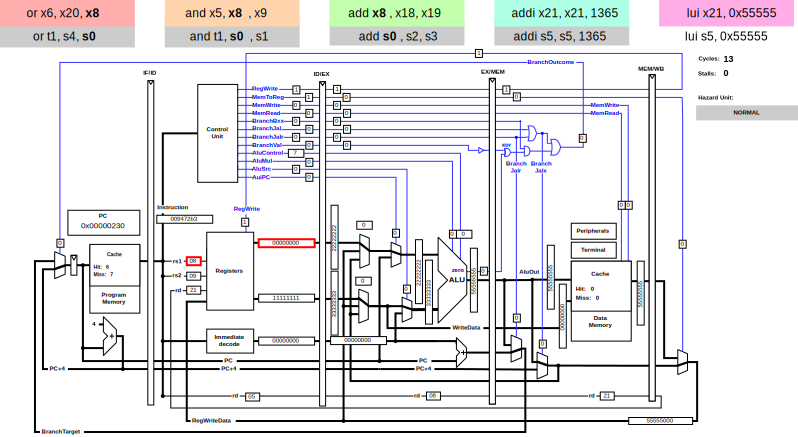
\includegraphics[width=0.95\textwidth]{hazard_forwarding.pdf}

{\tiny
QtRvSim \url{https://github.com/cvut/qtrvsim}
}

{\Tiny
\url{https://gitlab.fel.cvut.cz/b35apo/stud-support/-/blob/master/seminaries/qtrvsim/hazards-from-lecture/alu-hazards.S}
}

\end{frame}

\begin{frame}
\frametitle{QtRvSim -- přeposílání vstupu instrukce "and" z MEM}
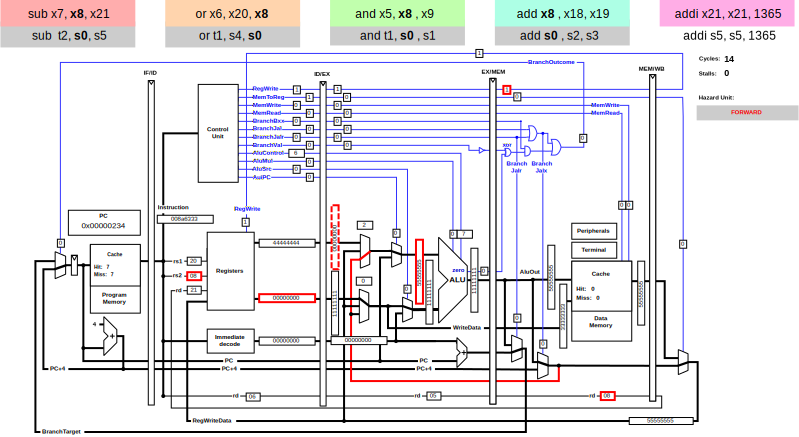
\includegraphics[width=0.95\textwidth]{hazard_forwarding2.pdf}

{\tiny
QtRvSim \url{https://github.com/cvut/qtrvsim}
}

{\Tiny
\url{https://gitlab.fel.cvut.cz/b35apo/stud-support/-/blob/master/seminaries/qtrvsim/hazards-from-lecture/alu-hazards.S}
}

\end{frame}

\begin{frame}
\frametitle{QtRvSim -- přeposílání vstupu instrukce "or" z WB}
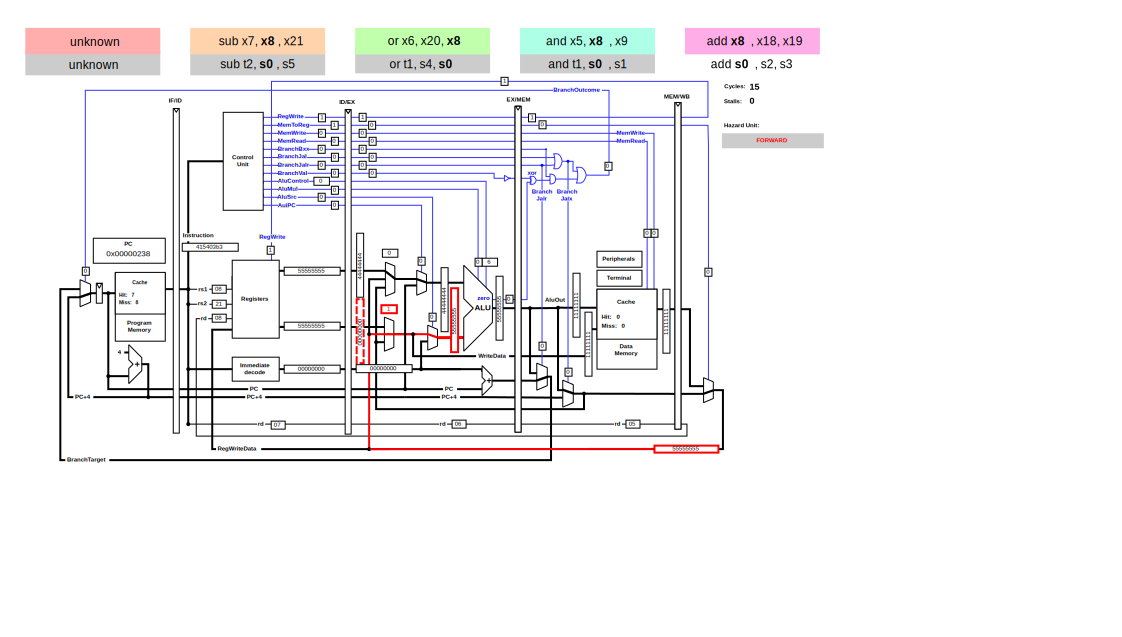
\includegraphics[width=0.95\textwidth]{hazard_forwarding3.pdf}

{\tiny
QtRvSim \url{https://github.com/cvut/qtrvsim}
}

{\Tiny
\url{https://gitlab.fel.cvut.cz/b35apo/stud-support/-/blob/master/seminaries/qtrvsim/hazards-from-lecture/alu-hazards.S}
}

\end{frame}

\begin{frame}
\frametitle{Přetrvávající problém v instrukci "lw" -- řešení pozastavení}
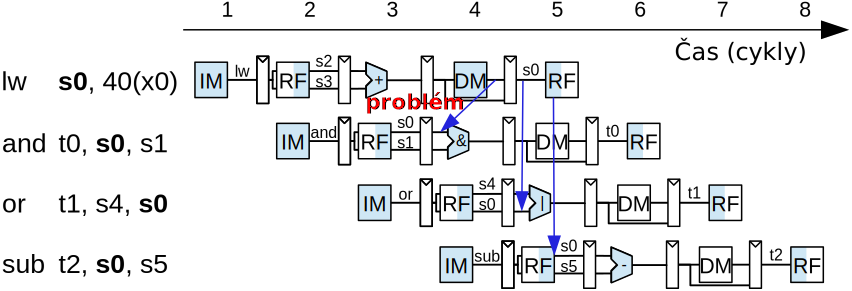
\includegraphics[width=0.85\textwidth]{pipeline_stall-cz.pdf}

\begin{itemize}
 \item Pokud následující instrukce vyžaduje data dříve, než jsou k dispozici v procesoru, tak je nutné
       pipeline pozastavit (\textbf{stall}) a do pokračování pipeline jsou vloženy stall/\textbf{nop}
       stavy
 \item Pozastavení řeší hazardy ale degraduje propustnost
 \item Stupně, které předchází stupni dotčenému hazardem, jsou pozastaveny, dokud nejsou všechny dalšími
       instrukcemi požadované výsledky k dispozici -- výsledky jsou pak přeposlané na všechna místa, kde
       jsou požadované
\end{itemize}

\end{frame}

\begin{frame}
\frametitle{Řešení datových hazardů pozastavením (pipeline stall)}
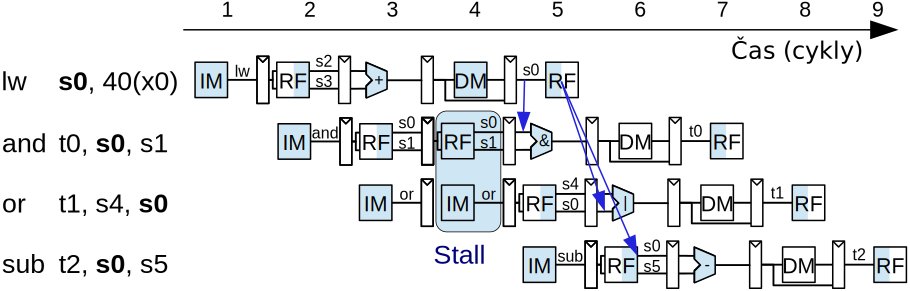
\includegraphics[width=0.85\textwidth]{pipeline_stall2-cz.pdf}

\begin{itemize}
 \item Pozastavení je realizované podržením obsahu mezistavových (interstage) registrů
       (hradlováním jejich hodinového signálu nebo nahrávacích signálů)
 \item Výsledky ze stupňů s chybějícími daty se nepoužijí, vynulují se signály
       pro zápis do paměti a registrů i ostatní řídicí signály
 \item Obojího je dosaženo přidáním řídicích signálů pro pozdržení a nebo
       nulování mezistupňových registrů
\end{itemize}

\end{frame}

\begin{frame}
\frametitle{Řešení zbývajících datových hazardů pozastavením}

\includegraphics[width=0.95\textwidth]{cpu_fwd_stall.pdf}
\end{frame}

\begin{frame}
\frametitle{QtRvSim -- datový hazard v "lw" řešený pozastavením}
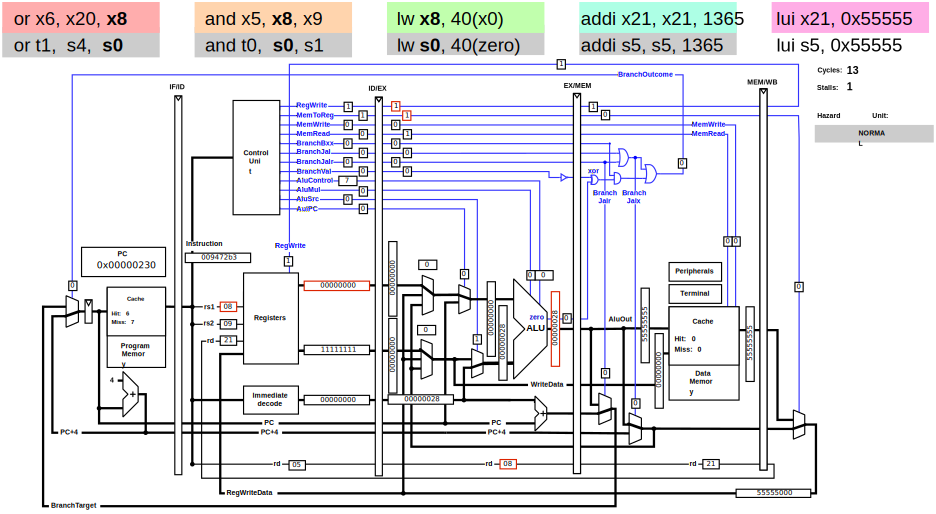
\includegraphics[width=0.95\textwidth]{hazard_stall_qtrvsim2.pdf}
{\tiny
QtRvSim \url{https://github.com/cvut/qtrvsim}
}

{\Tiny
\url{https://gitlab.fel.cvut.cz/b35apo/stud-support/-/blob/master/seminaries/qtrvsim/hazards-from-lecture/lw-hazards.S}
}

\end{frame}

\begin{frame}
\frametitle{QtRvSim -- datový hazard v "lw" řešený pozastavenímm}
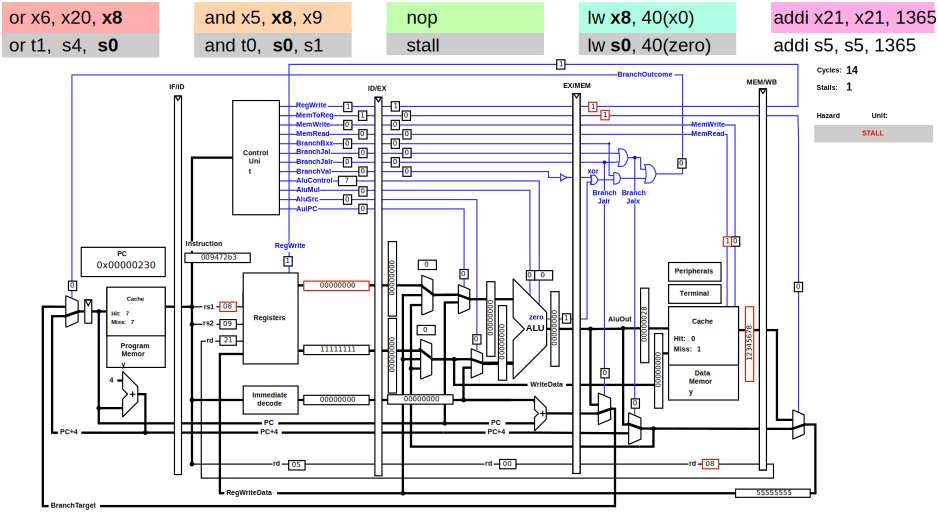
\includegraphics[width=0.95\textwidth]{hazard_stall_qtrvsim3.pdf}

{\tiny
QtRvSim \url{https://github.com/cvut/qtrvsim}
}

{\Tiny
\url{https://gitlab.fel.cvut.cz/b35apo/stud-support/-/blob/master/seminaries/qtrvsim/hazards-from-lecture/lw-hazards.S}
}

\end{frame}

\begin{frame}
\frametitle{QtRvSim -- datový hazard v "lw" řešený pozastavením}
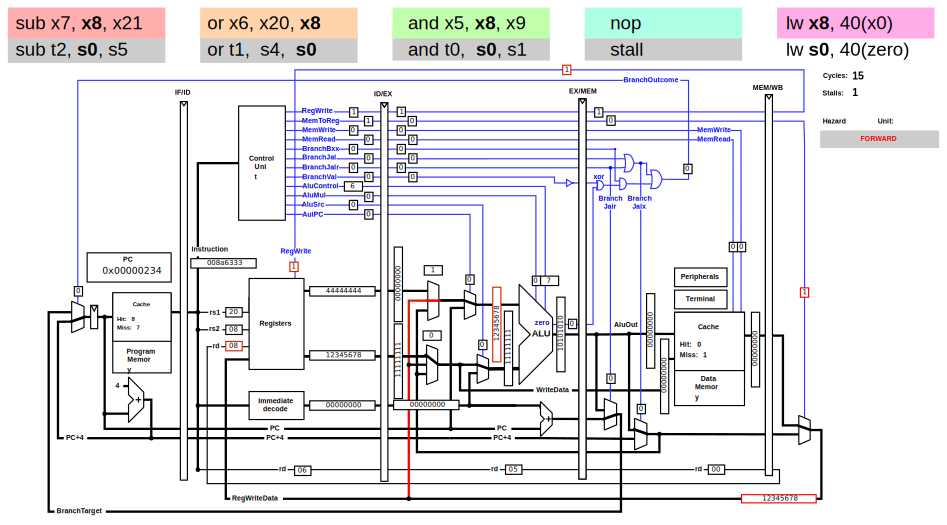
\includegraphics[width=0.95\textwidth]{hazard_stall_qtrvsim4.pdf}

{\tiny
QtRvSim \url{https://github.com/cvut/qtrvsim}
}

{\Tiny
\url{https://gitlab.fel.cvut.cz/b35apo/stud-support/-/blob/master/seminaries/qtrvsim/hazards-from-lecture/lw-hazards.S}
}

\end{frame}

\section{Řídící hazardy}

\begin{frame}
\frametitle{Řídicí (control) hazardy (instrukce branch a jump)}
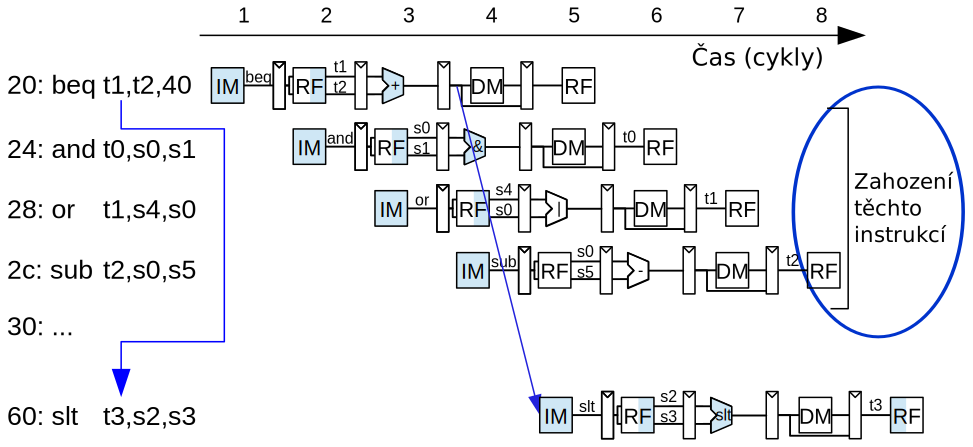
\includegraphics[width=0.85\textwidth]{hazard_ctrl-cz.pdf}

\begin{itemize}
 \item Výsledek není známý dříve než ve čtvrtém cyklu, poté se nahraje do PC
       a tak první instrukce na cílové adrese skoku může být načtena až v cyklu pátém
 \item Skoky takto představují zásadní omezení využití času výkonných jednotek v pipeline
\end{itemize}

\end{frame}

\begin{frame}
\frametitle{Alternativa, přesunout rozhodování skoků dříve}
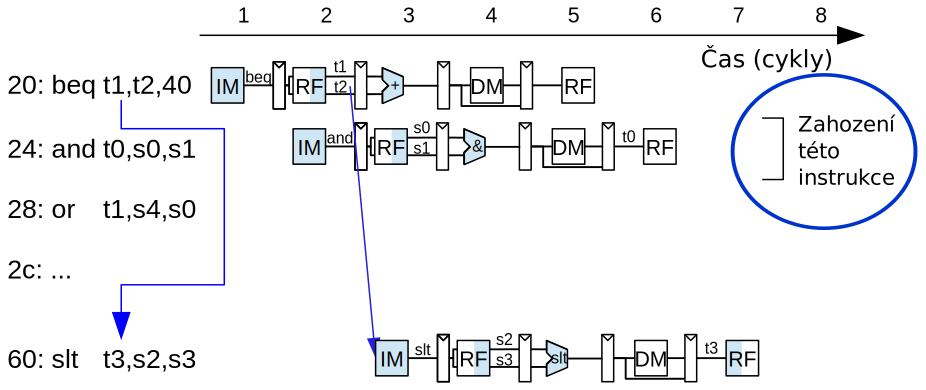
\includegraphics[width=0.85\textwidth]{hazard_ctrl2-cz.pdf}

\begin{itemize}
 \item Vzniká strukturální hazard, \textbf{ALU} je potřeba ve stupni \textbf{EX} i \textbf{ID}.
 \item Strukturální hazardy lze řešit duplikací prvků. Kompletní sčítačka, odčítačka nebo porovnání
       na velikost trvá dlouho, řešením může být omezit podmíny skoků jen na shodu/neshodu (stačí xor
       mezi operandy a nor přes bity)
\end{itemize}

\end{frame}

\begin{frame}
\frametitle{Přesun vykonání skoků do ID -- architektura MIPS}
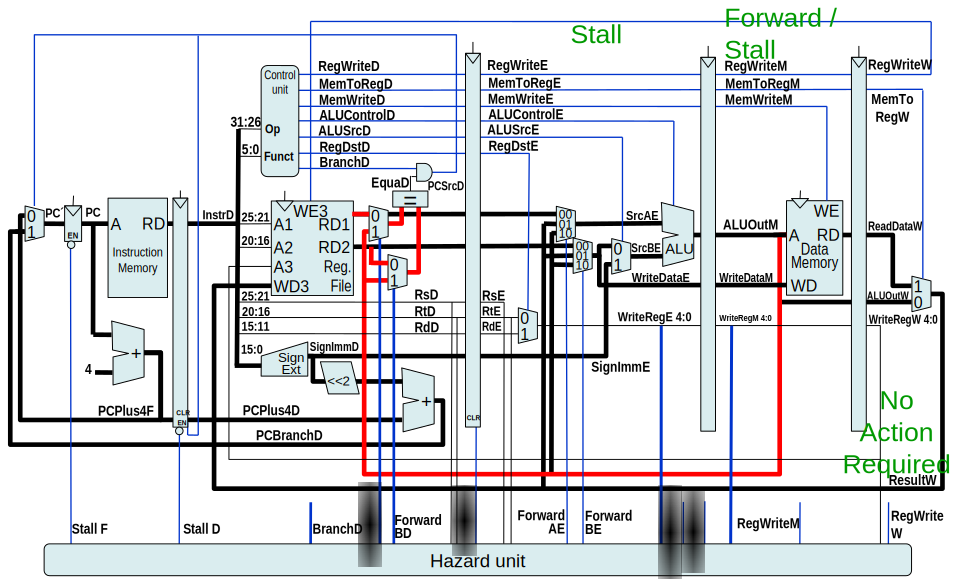
\includegraphics[width=0.90\textwidth]{hazard_ctrl_mips2.pdf}
\end{frame}

\begin{frame}
\frametitle{Vyřešení hazardů na vstupech komparátoru -- MIPS}
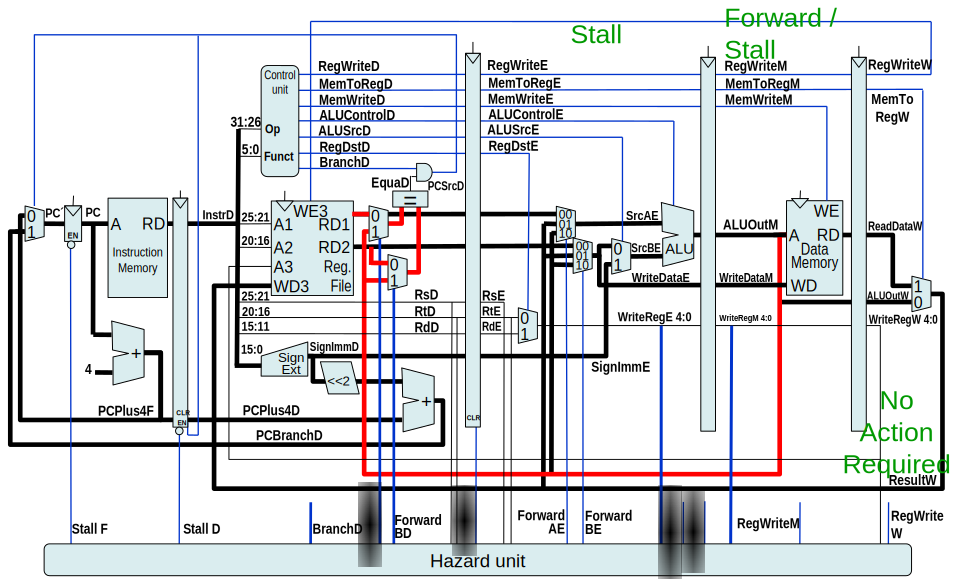
\includegraphics[width=0.90\textwidth]{hazard_ctrl_mips2.pdf}
\end{frame}

\begin{frame}
\frametitle{Predikce skoků a spekulativní vykonávání instrukcí (příště)}

\includegraphics[width=0.90\textwidth]{cpu_branch_pred.pdf}
\end{frame}

\begin{frame}
\frametitle{Výsledek návrhu zřetězeného procesoru -- RISC-V}

\includegraphics[width=0.95\textwidth]{cpu_final_design.pdf}
\end{frame}

\begin{frame}
\frametitle{Propustnost navrženého zřetězeného procesoru}

\begin{itemize}
 \item Jaká bude maximální dosažitelná frekvence procesoru?
 \item Který stupeň je nejpomalejší?
 \item Minimální přípustná perioda cyklu je daná nejpomalejším stupněm
 \item V našem případě se jedná o paměti \\
       $T_C = 300$\,ns $\rightarrow$ $f_{clk\,max} = 3\,333$\,kHz \\
       pokud neuvažujeme cykly navíc na plnění pipeline (žádná pozastavení
       a vyprázdnění například při skocích) tak pro ideální $IPC = 1$ \\
       $IPS = 1 \cdot 3\,333e3 = 3\,333\,000$ instrukcí za sekundu
 \item Zavedení pětistupňového zřetězeného zpracování vedlo k zvýšení
       propustnosti $3\,333\,000 / 980\,000 = 3.4 \times$ za předpokladu $IPC = 1$
\end{itemize}

\end{frame}

\section{Procesor s pamětí}

\begin{frame}
\frametitle{Jak koresponduje návrh s reálným procesorem s připojenou pamětí (pro zjednodušení neuvažujeme pipeline)}

\includegraphics[width=0.95\textwidth]{cpu_design.pdf}
\end{frame}

\begin{frame}
\frametitle{Pamět již nebudeme uvažovat na čipu}

\includegraphics[width=0.95\textwidth]{cpu_design2.pdf}
\end{frame}

\begin{frame}
\frametitle{Vracíme se k původnímu rozdělení procesor, paměť}

\includegraphics[width=0.85\textwidth]{cpu_design3.pdf}
\end{frame}

\begin{frame}
\frametitle{Která instrukce selže při přerušení spoje}
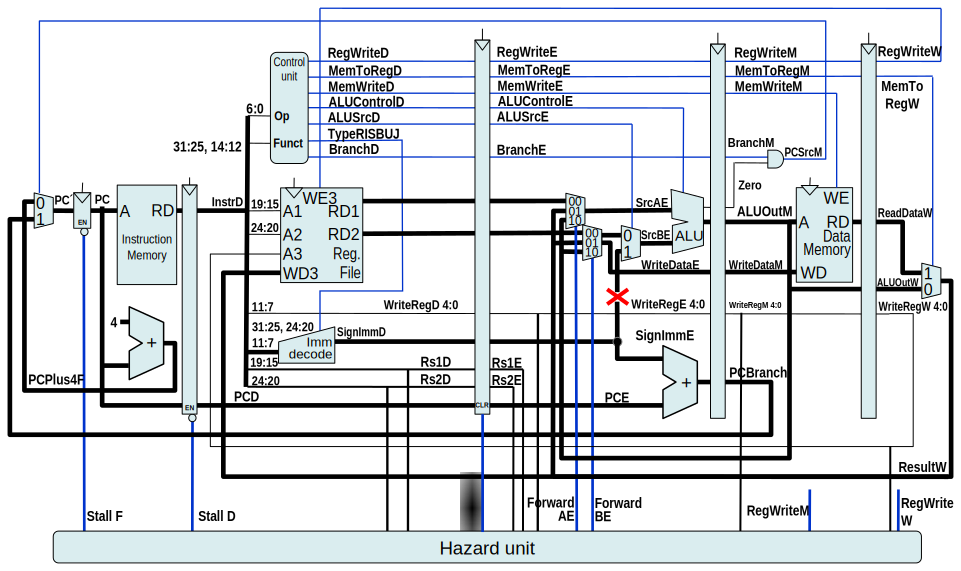
\includegraphics[width=0.95\textwidth]{cpu_final_design_bonus.pdf}

\textbf{A)} add \hfill \textbf{B)} addi \hfill \textbf{C)} beq \hfill \textbf{ D)} or \hfill ?
\end{frame}

\section{Úvahy a omezení pro reálný návrh (pro adepty na známku A)}

\begin{frame}
\frametitle{Requirements for Pipeline Timing}
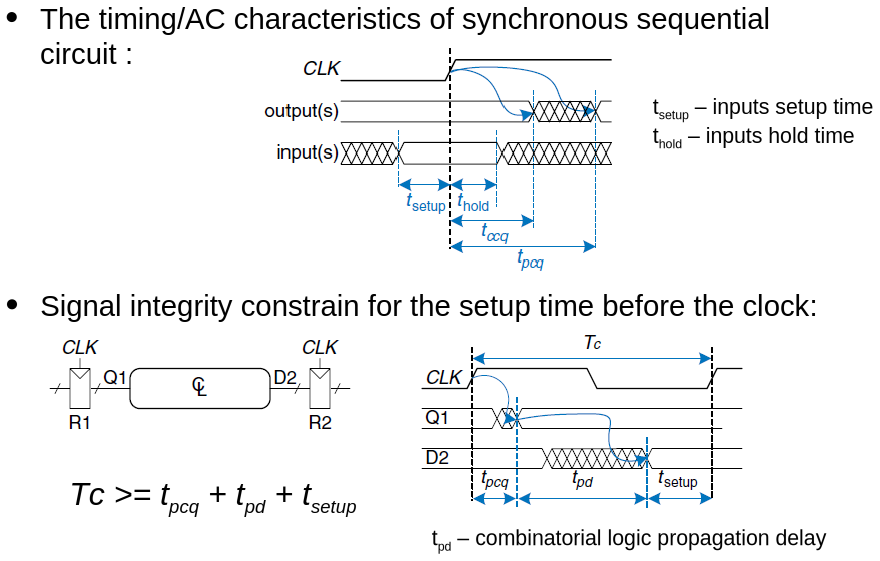
\includegraphics[width=0.95\textwidth]{pipeline_timing1.pdf}
\end{frame}

\begin{frame}
\frametitle{Requirements for Pipeline Timing}
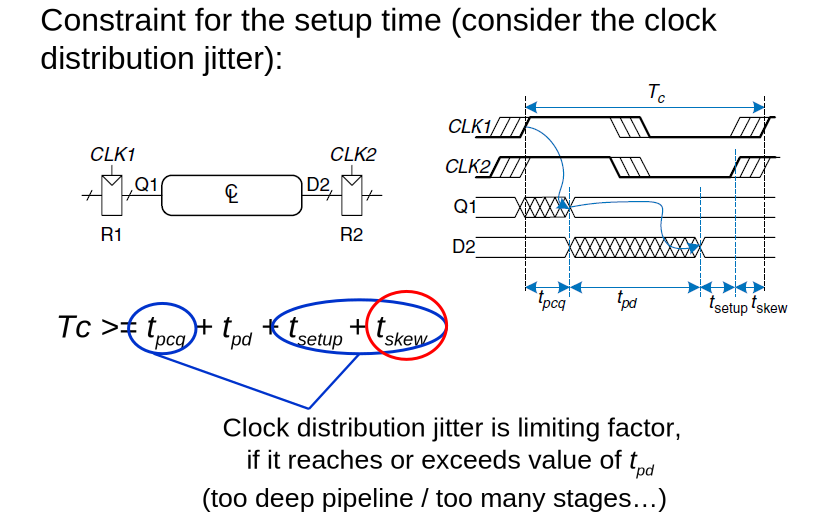
\includegraphics[width=0.95\textwidth]{pipeline_timing2.pdf}
\end{frame}

\begin{frame}
\frametitle{Clock Distribution Network Skew}
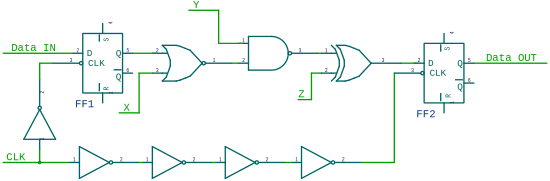
\includegraphics[width=0.9\textwidth]{clock_distribution_skew.pdf}

\begin{itemize}
 \item \textbf{Positive Clock Skew} -- clock arrives at the capturing sequential later than it arrives at the launching sequential
 \item \textbf{Negative Clock Skew} -- clock arrives at the launching sequential later than it arrives at the capturing sequential
 \item \textbf{Local Clock Skew} -- skew between any two sequentials with a valid timing path between them.
 \item \textbf{Global Clock Skew} -- clock skew between any two sequentials in the design irrespective of whether a timing paths exists between them
\end{itemize}

\end{frame}

\begin{frame}
\frametitle{Clock Distribution Network -- H-tree}

{
\centering
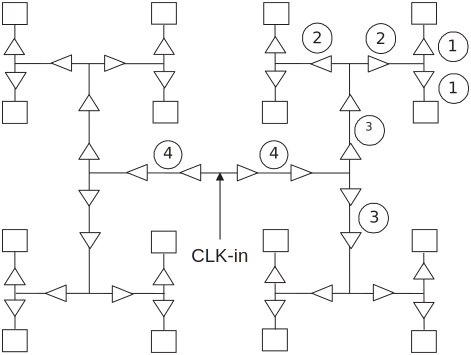
\includegraphics[width=0.6\textwidth]{clock_distribution_h_tree.pdf}
}

\vskip 2mm

source: Tawfik, S., Kursun, V.: Clock Distribution Networks with Gradual Signal Transition Time Relaxation for Reduced Power Consumption.

\end{frame}

\begin{frame}
\frametitle{Pipeline Stages Balancing}

\includegraphics[width=0.85\textwidth]{pipeline_balancing.pdf}

(applies to tree based adder, multiplier, (unrolled) iterative divider..)

\begin{itemize}
 \item \textbf{Balancing}: the goal is to divide the processing into N stages in such way, that stage propagation delays are roughly the same...
 \item The number of stages reflects preference of \underline{performance} (\underline{throughput}) versus latency.
\end{itemize}

\end{frame}

\begin{frame}
\frametitle{Superpipeline and Beyond}

\begin{itemize}
 \item Not well balanced 5-stage pipeline:
\end{itemize}


\includegraphics[width=0.85\textwidth]{pipeline_balancing2.pdf}

\begin{itemize}
 \item Deeper pipeline is result of decomposing stages into more stages
\end{itemize}


\includegraphics[width=0.85\textwidth]{pipeline_balancing3.pdf}

\begin{itemize}
 \item It allows CPU to work at higher frequencies but introduces many problems as well...
 \item Complex forwarding, more pipeline stalls, hazards need to be solved by complex logic
\end{itemize}

\end{frame}

\begin{frame}
\frametitle{Superpipeline and Beyond}


\includegraphics[width=0.95\textwidth]{pipeline_today_depths.pdf}

The Optimum Pipeline Depth for a Microprocessor: {\tiny \url{http://citeseerx.ist.psu.edu/viewdoc/download?doi=10.1.1.93.4333&rep=rep1&type=pdf}}

\end{frame}

\end{document}

